\documentclass[11pt,oneside]{article}
\usepackage{amsmath}
\usepackage{pdfpages}
\usepackage{appendix}
\usepackage{natbib}
% \usepackage{amssymb}
\usepackage{makeidx}
\usepackage{graphicx}
\usepackage{epstopdf}
\usepackage{float}
\usepackage{mdwlist}
\usepackage{bm}
\usepackage{fullpage}

\begin{document}
\title{Exploring non-linear inversions: a 1D magnetotelluric example}
\author{Seogi Kang, Lindsey Heagy, Rowan Cockett, and Douglas Oldenburg}

\maketitle

At some point in many geophysical workflows, an inversion is a necessary step for answering the geoscientific question at hand: whether it is recovering a reflectivity series from a seismic trace in a deconvolution problem, finding a susceptibility model from magnetic data or recovering conductivity from an electromagnetic survey. This is particularly true when working with data sets where it may not even be clear how to plot the data: 3D direct current resistivity and induced polarization surveys (it is not necessarily clear how to organize data into a pseudosection) or multi-component data, such as electromagnetic data (we can measure three spatial components of electric and/or magnetic fields through time over a range of frequencies). Inversion is a tool for translating these data into a model we can interpret. The goal of the inversion is to find a ``model'', some description of the earth’s physical properties, that is consistent with those data and geologic knowledge.

In spite the wide applicability of inverse problems, inversions are often used (and provided) as black-boxes: data goes in, some number crunching happens, your computer fan starts working pretty hard, and at some point a list of numbers (the model) comes out the other side. In such a paradigm, it is often unclear how to set expectations of what information we should be able to extract from our data through inversion, and difficult to gauge how to use all of the knobs appropriately (trade-off parameters, stopping criteria, noise model, choice of regularization functional, mesh generation, etc.).

A number of authors have published tutorials and papers that open up the black box and discuss the numerical gears that make an inversion machine run as well as the knobs that tune it. \cite{OldenburgTutorial} provides a comprehensive tutorial on inversion; many of the topics we will discuss are presented in much more detail in their tutorial. The implementation of the physics simulations, optimization, and structure necessary to perform an inversion can be overwhelming to implement and organize from scratch; in \citep{SimPEGPaper}, we introduce a general simulation and inversion framework and a set of tools (in Python!) to hopefully make this easier.

The style of the Leading Edge tutorials ups the ante, as we can provide code that brings examples to life so that not only can you see images produced by someone else, you can play with the knobs yourself. Matt Hall kicked off the discussion of inversions in the Leading Edge in his \emph{Linear Inversion} tutorial \citep{HallTutorial}. He walked through how to solve the classic linear inverse problem $\mathbf{G}\mathbf{m} = \mathbf{d}$, where $\mathbf{G}$ is our forward operator (the mathematical description of the physics/problem), $\mathbf{d}$ is our data, and $\mathbf{m}$ is what we are after: our ``model'' of the earth. The example he demonstrated is a deconvolution problem, in that case, $\mathbf{G}$ is a convolution matrix, $\mathbf{m}$ is the reflectivity series and $\mathbf{d}$ is a seismic trace. He introduced the concepts of an underdetermined problem, motivated the need for regularization, formulated the inversion in terms of an optimization problem and solved the linear inverse problem (in true polyglot fashion, using Python, Lua, Julia, and R!).

\section{Magnetotellurics}
In this tutorial, we will pick up from there and explore a nonlinear forward problem, of the form $\mathcal{F}[\mathbf{m}] = \mathbf{d}$. Here, we choose $\mathcal{F}[\mathbf{m}]$ to be the 1D magnetotelluric (MT) forward simulation. The MT problem is a natural source electromagnetic method; plane-wave source-fields are generated by solar wind (giving us low frequency signals $<$ 1 Hz) and lightning strikes worldwide (giving us higher frequency signals $>$ 1 Hz). In magnetotellurics, the model, $\mathbf{m}$, is a description of the earth’s electrical conductivity and $\mathcal{F}[\mathbf{m}]$ solves Maxwell’s equations for a plane wave source:
\begin{equation}
\begin{split}
\nabla \times \vec{E} + i\omega\mu\vec{H} &= 0 \\
\nabla \times \vec{H} + \sigma\vec{E} &= 0
\end{split}
\label{eq:maxwell}
\end{equation}
The plane wave source is incorporated in the modelling through a boundary condition. The data, $\mathbf{d}$, are impedances; for the 1D problem, the impedance at a single frequency is given by
\begin{equation}
Z_{xy} = -\frac{E_x}{H_y}.
\label{eq:impedance}
\end{equation}
Note that the impedance is a complex number. When we work with the data in the inversion, it is convenient to work only with real numbers, so at each frequency we define 2 data points: $\text{Re}(Z_{xy})$ and $\text{Im}(Z_{xy})$, thus the total number of data for the 1D simulations we will consider are $2 \times N_{\text{frequencies}}$. Impedance is a non-intuitive quantity; often, we instead consider apparent resistivity\footnote{Note that resistivity is the inverse of conductivity $\rho = 1/\sigma$} and phase, given by
\begin{equation}
\rho_a = \frac{1}{\mu_0\omega} \big|Z_{xy}\big|^2,
\quad
\phi = \tan^{-1}\left(\frac{\text{Im}(Z_{xy})}{\text{Re}(Z_{xy})}\right).
\label{eq:rhoa_phase}
\end{equation}
For an earth that is a half-space, the apparent resistivity equals the true resistivity, and the phase is $45^{\circ}$. The ability to compute the complex impedance or apparent resistivity and phase solves the forward problem.

The inversion aims to solve $\mathcal{F}^{-1}[\mathbf{d}]$ for a model. Just as in the linear problem, we are dealing with an ill-posed inverse problem\footnote{Ill posed problems are problems that are not well-posed. For a well-posed problem, a solution exists, the solution is unique and the solution depends continuously on the input.}, thus, regularization is required in order to select a model from the infinitely many that can fit the data. Before we tackle the inverse problem, let's explore an example of nonuniqueness: how can different models give us the same data?

\section{Go forwards}
Prior to any inversion, we require the ability to accurately simulate predicted data. In a few specific cases, this can be accomplished by analytically solving a set of equations with the specified boundary conditions, but in general, we must discretize the equations of interest (here, Maxwell’s equations) and solve the partial differential equations. In the first notebook, we walk through a finite difference approach for solving the 1D MT problem. Rather than going into those details in this write up, we will let you explore the notebook, and if you are looking for more, we wrote a tutorial on finite volume methods \citep{Cockett2016}! Here, we take for granted that we have designed an appropriate mesh\footnote{The mesh must extend far enough so that the lowest frequency electromagnetic fields have decayed sufficiently by the time they reach it, and the finest cells must be small enough as to capture the behaviour of the highest frequencies. See the second notebook for more discussion.}, can solve Maxwell’s equations, and will use forward modelling as a tool for setting expectations on what we can hope to recover from our data. In particular, let’s examine an example of nonuniqueness.

A classic example that demonstrates non-uniqueness of MT data is the equivalence of the   conductivity-thickness product (conductance) of a thin layer. If we start with a layer that has a conductivity of $\sigma$, halve its thickness and double its conductivity, the resulting data will be similar. In Figure \ref{fig:sigmat}, we show apparent resistivity and phase data for five models, each of which has the same conductance. In all of the simulations, the data shows a decrease in apparent resistivity and an increase in phase starting at $\sim$10Hz. Thus in all of the data we have evidence of a conductive layer, and the frequency range at which it appears is an indicator of the depth of the layer (you can explore by changing the \texttt{depth} variable in the model setup of the second notebook). However, all scenarios produce similar data, and in the second interactive notebook, you can explore what happens if you add noise. Even with a small amount of noise, we cannot expect an inversion code to separate the conductivity and thickness of a conductive unit without incorporating additional information. When setting up the inverse problem and defining regularization (next up!), it is important to realize that the choices we make there will influence the character of the model we recover, as the data alone do not provide us with a unique model.

\begin{figure}[htb!]
    \centering
    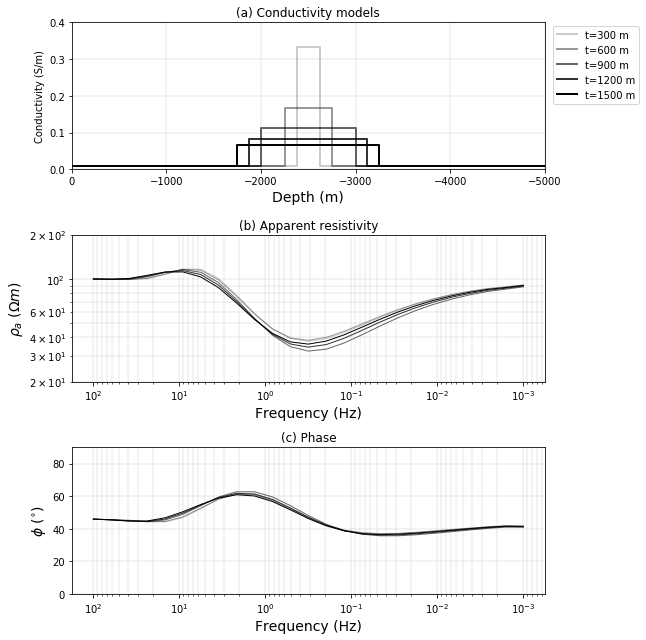
\includegraphics[width=\textwidth]{../images/sigmat_old.png}
\caption{Magnetotelluric responses from five models, each having an equivalent conductivity-thickness product for the conductive layer. (a) Conductivity models, (b) apparent resistivity ($\rho_a$), and (c) phase ($\phi$).}
\label{fig:sigmat}
\end{figure}

\section{Go backwards}

To solve the inverse problem, we will use a deterministic approach and pose the inverse problem as an optimization problem of the form
\begin{equation}
\min_{\mathbf{m}} \phi(\mathbf{m}) = \phi_d(\mathbf{m}) + \beta\phi_m(\mathbf{m})
\end{equation}
where $\mathbf{m}$ is our model - the array of numbers that describes our earth model; $\phi_d(\mathbf{m})$ is the data misfit, a measure of ``how far'' our data are from the observed data; $\phi_m(\mathbf{m})$ is the regularization; and $\beta$ is a trade-off parameter.

The data misfit, is often taken to be a weighted $\ell_2$-norm:
\begin{equation}
\phi_d(\mathbf{m}) = \frac{1}{2}\|\mathbf{W_d} (\mathcal{F}(\mathbf{m}) - \mathbf{d}^{\text{obs}})\|^2
\end{equation}
where $\mathbf{W_d}$ captures the noise model (typically it is a diagonal matrix containing the standard deviation of each datum). Tikhonov regularization, which again employs $\ell_2$-norms, is a standard choice:
\begin{equation}
\phi_m(\mathbf{m}) = \frac{1}{2}\big(\alpha_s\|\mathbf{W_s} (\mathbf{m} - \mathbf{m}_{\text{ref}})\|^2 + \alpha_z\|\mathbf{W_z} (\mathbf{m})\|^2 \big)
\end{equation}
The first term is often referred to as the "smallness" as it measures the "size" of the model (in the $\ell_2$ sense). The matrix $\mathbf{W_s}$ is generally taken to be a diagonal matrix that may contain information about the length scales of the model or be used to weight the relative importance of various parameters in the model. The scalar $\alpha_s$ weights the relative importance of this term in the regularization. Notice that we include a reference model, $\mathbf{m}_{\text{ref}}$. Often this is defined as a constant value, but if more information is known about the background, that can be used to construct a more intricate reference model. Here, we will not delve too far into how the reference model impacts the recovered results, but you are encouraged to change \texttt{mref} in the notebooks and investigate its impact. The second term is often referred to as the "smoothness". The matrix $\mathbf{W_z}$ approximates the derivative of the model with respect to depth, and is hence a measure of how "smooth" the model is. The term $\alpha_z$ weights the relative importance of smoothness in the regularization.

From this setup, we see that there are quite a number of choices to make: defining uncertainties on the data ($\mathbf{W_d}$), selecting a reference model ($\mathbf{m}_{\text{ref}}$), choosing the importance of smallness and smoothness ($\alpha_s$ and $\alpha_z$), and selecting a trade-off parameter ($\beta$). Let’s start by assuming a known noise model, fix $\alpha_s$ and $\alpha_z$, and explore the impact of the trade off parameter $\beta$. Our forward problem depends upon the electrical conductivity. For the inverse problem, however, we are free to use any function of the conductivity as a parameter. The electrical conductivity of earth materials varies by many orders of magnitude and is strictly positive. Thus it is advantageous to use $\mathbf{\log(\sigma)}$ as the model in the inverse problem. For a nonlinear problem, we also have the additional choice of the initial model $\mathbf{m}_0$ at which to start the inversion. Although we will not discuss the choice of $\mathbf{m}_0$, you are encouraged to change the initial model in the notebooks and examine the impact it makes - it can be significant!

\subsection{The $\beta$ knob}

If the noise is Gaussian, then the sum of squares (our data misfit) is a Chi-squared distribution, which has an expected value of $N_\text{data}$ (in our case, we divide this by two to match our definition of $\phi_d$). Thus, the ideal choice of $\beta$ is one that gives us $\phi_d^* \approx \frac{1}{2} N_\text{data}$. To demonstrate the effect of $\beta$, we consider a five layer model, originally shown in \cite{Monographs}, and will demonstrate inversions when we achieve the target misfit, underfit the data and overfit fit the data. The conductivity model used is the solid line in Figure \ref{fig:justright}a. For these inversions we fix the regularization parameters to $\alpha_s = 10^{-2}$, $\alpha_z = 1$ and set $\mathbf{m}_{\text{ref}} = 10^{-2} S/m$, and the initial model, $\mathbf{m}_0 = \mathbf{m}_{\text{ref}}$ (feel free to change them in the notebook!). We start the inversion with a large $\beta$ and decrease its value to plot the trade-off or Tikhonov curve (Figure \ref{fig:justright}b). In this figure, the inversion is stopped when the data misfit approximately equals the  target misfit (the star in Figure \ref{fig:justright}b). Figures \ref{fig:justright}c and \ref{fig:justright}d show the data as apparent resistivity and phase, which is a visualization of our complex-valued impedance data. The dashed line in Figure \ref{fig:justright}a shows the recovered model, which identifies the general structure and amplitudes of the five layer model. In this case, we are employing a smooth regularization, thus we expect to recover smoothly varying structures.



\begin{figure}[htb!]
    \centering
    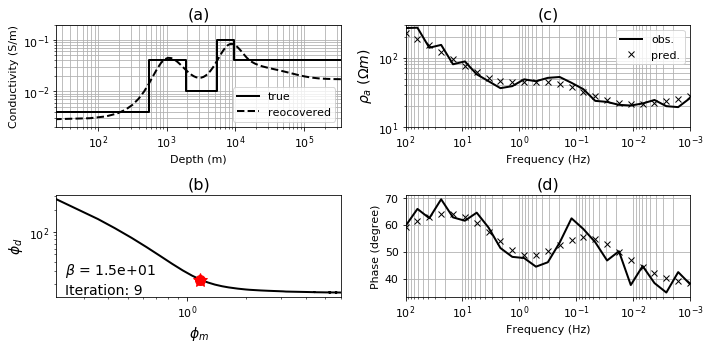
\includegraphics[width=\textwidth]{../images/justright_old.png}
\caption{Inversion which achieves target misfit. (a) True (solid) and recovered (dashed) electrical conductivity models. (b) Tikhonov curve showing the target misfit (red star) and achieved misfit (red circle, in this example they overlap) in the inversion (c) observed (solid) and predicted (x’s) apparent resistivity data, (d) observed (solid) and predicted (x’s) phase data}
\label{fig:justright}
\end{figure}

If we instead choose a larger $\beta$, reducing the contribution of the data misfit to the objective function, we ``underfit'' the data, as is shown in Figure \ref{fig:underfit}. Although we still see evidence of two conductive structures, we do not recover their amplitudes, and do a poor job resolving the location and widths of the conductive layers (if you had to pick the top of the first layer - where should it be?). Examining the data plots in \ref{fig:underfit}c and d, there is more insight about the subsurface conductivity that can be learned by extracting more information from the data.


\begin{figure}[htb!]
    \centering
    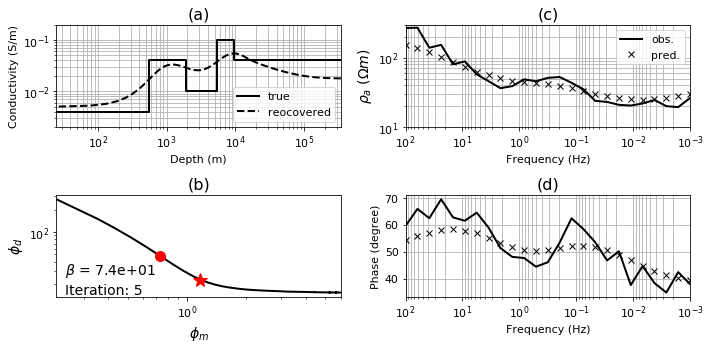
\includegraphics[width=\textwidth]{../images/underfit_old.png}
\caption{Inversion which underfits the data. (a) True (solid) and recovered (dashed) electrical conductivity models. (b) Tikhonov curve showing the target misfit (red star) and achieved misfit (red circle) in the inversion (c) observed (solid) and predicted (x’s) apparent resistivity data, (d) observed (solid) and predicted (x’s) phase data}
\label{fig:underfit}
\end{figure}

On the other extreme, we can choose a very small $\beta$, and try to fit all of the details in the data. Doing this, we obtain the results shown in Figure \ref{fig:overfit}. When we push the inversion to fit the (noisy!) data very closely, we end up fitting the noise. In order to do this, conductivity contrasts are exaggerated and oscillatory and erroneous conductivity structures are introduced in the inversion.



\begin{figure}[htb!]
    \centering
    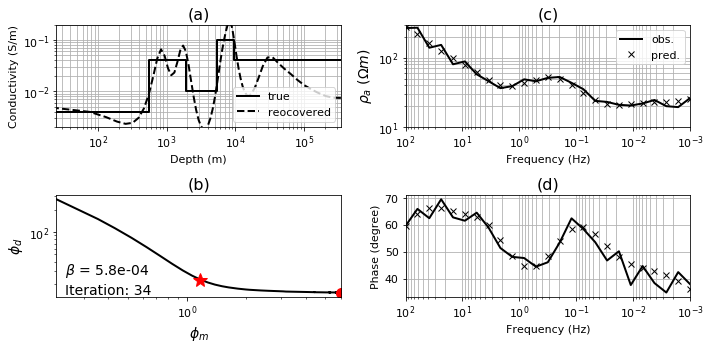
\includegraphics[width=\textwidth]{../images/overfit_old.png}
\caption{Inversion which overfits the data. (a) True (solid) and recovered (dashed) electrical conductivity models. (b) Tikhonov curve showing the target misfit (red star) and achieved misfit (red circle) in the inversion (c) observed (solid) and predicted (x’s) apparent resistivity data, (d) observed (solid) and predicted (x’s) phase data}
\label{fig:overfit}
\end{figure}
\subsection{The $\alpha$ knobs}

For Figures \ref{fig:justright}-\ref{fig:overfit}, we prescribed the values the $\alpha_s$, $\alpha_z$. What impact do they have on the character of the model we recover?

In Figure \ref{fig:alphas}, we compare two inversions with different regularization parameters: (1) a ``smooth'' inversion (blue line), with $\alpha_s = 10^{-5}$ and $\alpha_z = 1$, and (2) a ``small'' inversion (red line): with $\alpha_s = 1$ and $\alpha_z = 10^{-5}$. In both, $\beta$ was chosen so that a desired target misfit was achieved. The smooth inversion penalizes large gradients; the resulting model has two smooth peaks. Note that we smooth over the resistive third layer, over-estimating its conductivity. The ``small'' inversion instead favors models that are close to the reference model; this model has more structure. The resistivity of the first layer matches well (the conductivity of the first layer is equivalent to our reference model) and the conductivity of the third layer is closer to its true value, but additional oscillatory structures are introduced at depth. In the fourth notebook, you can explore the impact of these parameters yourself!

\begin{figure}[htb!]
    \centering
    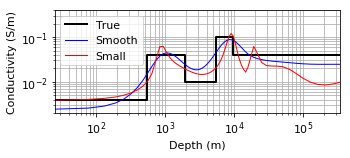
\includegraphics[width=0.5\textwidth]{../images/alphas_old.png}
\caption{Comparing the use of Smooth regularization versus Small regularization in the inversion.}
\label{fig:alphas}
\end{figure}


In practice, these parameters are often determined by experimentation; strategies such as examining length scales are often successfully adopted (see page 38 \cite{OldenburgTutorial}). Changing the relative values of $\alpha_s$ and $\alpha_z$ is one way to bring in a-priori information, if we know very little, often starting with a smooth inversion is a good option; this penalizes structure (high gradients) while showing general trends. If more structure is expected, or a reliable reference model can be built from additional data such as physical property measurements, well logs, or additional geophysical/geologic data, then the influence of the smallness term may be increased. There are a few other ways to bring in additional a-priori information. If we are expecting a more ``blocky'' model, we can choose a different norm (such as an $\ell_1$ norm), or if we have structural constraints, we can introduce other weighting structures (e.g. on the smoothness); these are knobs for another tutorial and there is discussion in \cite{OldenburgTutorial}.

\section{Summary}
In this tutorial, we have introduced the forward simulation of Maxwell’s equations for magnetotellurics and explored a few aspects of the inverse problem. Prior to jumping into an inversion, it is important to know the limitations of the survey and data and what you can and cannot resolve, even if there is no noise! Forward modelling is a powerful tool for setting realistic expectations of an inversion. In the magnetotelluric problem, thin layers which have the same conductance produce very similar data signatures and we cannot expect to independently resolve both the conductivity and thickness of a layer without bringing in additional information.

To set up and solve the inverse problem, we introduced a simple deterministic inversion for the electrical conductivity where we posed the inversion as an optimization problem that minimizes an objective function consisting of a data misfit and a regularization term. There are many choices to be made in defining the various elements of the inverse problem, including how to assign uncertainties, selecting a trade-off parameter, defining the regularization function, and choosing an initial and reference model. In this tutorial we explored two of the knobs: (1) the trade-off parameter and (2) the relative importance of smallness and smoothness contributions in a Tikhonov regularization. There are many other parameters that can be introduced, tuned and manipulated -- this should first be done with a synthetic, when you know the true model! The interactive notebooks that are provided allow you to change parameters and experiment with their impact.

\clearpage
\bibliographystyle{seg}  % style file is seg.bst
\bibliography{references.bib}

\end{document}
